
\documentclass[twoside]{ctuthesis}



\usepackage{textcomp}
\usepackage{xfrac}
\usepackage{algorithm,algorithmic}
\usepackage{caption}
\usepackage{subcaption}
\usepackage[colorinlistoftodos,prependcaption]{todonotes} %textsize = tiny option
\usepackage{xargs}                      % Use more than one optional parameter in a new commands
%\usepackage[dvipsnames]{xcolor}  % Coloured text etc.
%\usepackage[unicode]{hyperref}
\newcommand{\spc}[2]{$\mathbb{#1}^{#2}$}
\newcommand{\minsp}[3]{$\mathbb{#1} \in \mathbb{#2}^{#3}$}
\newcommand{\tl}[1]{$\mathbf{#1}$}
\newcommand{\tli}[2]{$\mathbf{#1}_{#2}$}
\newcommand{\norm}[1]{\left\lVert#1\right\rVert}
\newcommandx{\unsure}[2][1=]{\todo[linecolor=red,backgroundcolor=red!25,bordercolor=red,#1]{#2}}
\newcommandx{\change}[2][1=]{\todo[linecolor=blue,backgroundcolor=blue!25,bordercolor=blue,#1]{#2}}
\newcommandx{\info}[2][1=]{\todo[linecolor=OliveGreen,backgroundcolor=OliveGreen!25,bordercolor=OliveGreen,#1]{#2}}
\newcommandx{\improvement}[2][1=]{\todo[linecolor=Plum,backgroundcolor=Plum!25,bordercolor=Plum,#1]{#2}}


\ctusetup{
	preprint = \ctuverlog,
%	mainlanguage = english,
    titlelanguage = czech,
	mainlanguage = czech,
	otherlanguages = {slovak,english},
	title-czech = {Detekce objektů z hloubkové kamery},
	title-english = {Object Detection from Depth camera},
	%subtitle-czech = {Cesta do tajů kdovíčeho},
	subtitle-english = {Journey to the who-knows-what wondeland},
	doctype = B,
	faculty = F3,
	department-czech = {Katedra kybernetiky},
	department-english = {Department of Cybernetics},
	author = {Lukáš Kunt},
	supervisor = {Dr. Petr Štěpán},
	supervisor-address = {Ústav X, \\ Uliční 5, \\ Praha 99},
	%supervisor-specialist = {John Doe},
	fieldofstudy-english = {Mathematical Engineering},
	subfieldofstudy-english = {Mathematical Modelling},
	%fieldofstudy-czech = {Matematcké inženýrství},
	subfieldofstudy-czech = {Kybernetika a robotika},
	keywords-czech = {slovo, klíč},
	keywords-english = {word, key},
	day = 11,
	month = 5,
	year = 2020,
	%specification-file = {ctutest-zadani.pdf},
%	front-specification = true,
%	front-list-of-figures = false,
%	front-list-of-tables = false,
%	monochrome = true,
%	layout-short = true,
}

\ctuprocess

\addto\ctucaptionsczech{%
	\def\supervisorname{Vedoucí}%
	\def\subfieldofstudyname{Studijní program}%
}

\ctutemplateset{maketitle twocolumn default}{
	\begin{twocolumnfrontmatterpage}
		\ctutemplate{twocolumn.thanks}
		\ctutemplate{twocolumn.declaration}
		\ctutemplate{twocolumn.abstract.in.titlelanguage}
		\ctutemplate{twocolumn.abstract.in.secondlanguage}
		\ctutemplate{twocolumn.tableofcontents}
		\ctutemplate{twocolumn.listoffigures}
	\end{twocolumnfrontmatterpage}
}

% Theorem declarations, this is the reasonable default, anybody can do what they wish.
% If you prefer theorems in italics rather than slanted, use \theoremstyle{plainit}
%\theoremstyle{plain}
%\newtheorem{theorem}{Theorem}[chapter]
%\newtheorem{corollary}[theorem]{Corollary}
%\newtheorem{lemma}[theorem]{Lemma}
%\newtheorem{proposition}[theorem]{Proposition}

%\theoremstyle{definition}
%\newtheorem{definition}[theorem]{Definition}
%\newtheorem{example}[theorem]{Example}
%\newtheorem{conjecture}[theorem]{Conjecture}

%\theoremstyle{note}
%\newtheorem*{remark*}{Remark}
%\newtheorem{remark}[theorem]{Remark}

%\setlength{\parskip}{5ex plus 0.2ex minus 0.2ex}

\begin{document}
\maketitle

%\part{Teoretická část}
%\chapter{Teoretická část}
\chapter{Matematický aparát}
\section{Homogenní souřadnice}
Během celé práce budu pracovat jak s kartézskými, tak i s homogenními souřadnicemi. Ty jsou v Euklidovském prostoru dimenze $n$ reprezentovány pomocí vektoru, který má $n+1$ prvků. Je-li $\boldsymbol{r}$ bod v trojdimenzionálním Euklidovském prostoru $\mathbb{E}^3$ reprezentován parametry $x,y,z$, pak pro převod mezi kartézskými a homogenními souřadnicemi platí následující vztahy.
\begin{align}
    \mathbf{r} = \begin{bmatrix} x \\ y \\ z \end{bmatrix} &\rightarrow \mathbf{r}_{hom} = \begin{bmatrix} x \\ y \\ z \\ 1 \end{bmatrix} \\
    \mathbf{r}_{hom} = \begin{bmatrix} x \\ y \\ z \\ w \end{bmatrix} &\rightarrow \mathbf{r} = \begin{bmatrix} \sfrac{x}{w} \\ \sfrac{y}{w} \\ \sfrac{z}{w} \end{bmatrix}
\end{align}
Pomocích homogenních souřadnic můžeme sestavit transformační matici \tl{A} , tato se skládá z matice rotace \tl{R} a vektoru translace \tl{t}.
\begin{align}
    \mathbf{A} = \begin{bmatrix} \mathbf{R} & \mathbf{t} \\ \mathbf{0} & 1 \end{bmatrix}
\end{align}

\section{Rotace a rotační matice}
Natočení souřadného systému, popřípadě objektu s tímto svázaným vhledem k jinému systému v prostoru dimenze $n$ se nejjednodušeji popíše pomocí rotační matice \tl{R} $\in$ \spc{R}{n}. Mezi nejběžnější rotační matice patří rotace o úhel $\theta$ kolem os kartézského souřadného systému v \spc{E}{3}. Tyto matice vypadají následovně.
\begin{align}
    \mathbf{R_x}=\begin{bmatrix} \cos \theta & -\sin \theta & 0 \\ \sin \theta & \cos \theta & 0 \\ 0 & 0 & 1 \end{bmatrix} \\
    \mathbf{R_y}=\begin{bmatrix} \cos \theta & -\sin \theta & 0 \\ \sin \theta & \cos \theta & 0 \\ 0 & 0 & 1 \end{bmatrix} \\
    \mathbf{R_z}=\begin{bmatrix} \cos \theta & -\sin \theta & 0 \\ \sin \theta & \cos \theta & 0 \\ 0 & 0 & 1 \end{bmatrix}
\end{align}
Obecné natočení pak můžeme dostat složením 3 a více těchto rotací \footnote{Na pořadí zde záleží. Není možné dostat libovolnou rotační matici, pokud budou dvě po sobě doucí rotace probíhat kolem stejné osy}
Pro vytvoření matice rotace \tl{R} v prostoru \spc{R}{3} kolem obecné osy dané normalizovaným vektorem \tl{u} o úhel $\theta$ slouží Rodriguesův vzorec \cite{RodriguesRotationFormula}.
\begin{align}
    \mathbf{R} = \mathbf{I} + \tilde{\mathbf{u}}\sin \theta + \tilde{\mathbf{u}}^2(1 - \cos \theta); \quad \tilde{\mathbf{u}} = \begin{bmatrix} 0 & -u_{z} & u_{y} \\ u_z & 0 & -u_x \\ -u_y & u_x & 0 \end{bmatrix}
    \label{Rodriguez}
\end{align}
Chceme-li natočit vektor \tl{a} tak, aby byl rovnoběžný s vektorem \tl{b}, použijeme vzorec \ref{Rodriguez}, úhel rotace $\theta$ a vektor $\tilde{\mathbf{u}}$, kolem kterého rotace proběhne, se určí následovně.
\begin{align}
    \tilde{\mathbf{u}} = \frac{\mathbf{a} \times \mathbf{b}}{\norm{\mathbf{a}\times \mathbf{b}}} \label{eq:vector_rogrig}\\
    \theta = \arccos \left( \frac{\mathbf{a} \cdot \mathbf{b}}{\norm{\mathbf{a}}\norm{\mathbf{b}}} \right) \label{eq:angle_rogrig}
\end{align}
Podle \cite{james_w_angle_2014} je tato metoda nevhodná pro výpočet na počítači. Zejména pak v případech, kdy bychom měli počícat $\arccos$ hodnot blízko $\pm 1$. Toto je způsobeno omezenou přesností reprezentace desetinných čísel v počítači (takzvaná floating point aritmetika). Přesnější je tedy použít tento vzorec.
\begin{align}
    \theta = \text{atan2}\left( \norm{\mathbf{a} \times \mathbf{b}}, \mathbf{a}\cdot \mathbf{b} \right) 
\end{align}
Výhoda funkce atan2 oproti arcus tangens je ošetřené dělení nulou, ke kterému může dojít při zaokrouhlování desetinných čísel. Navíc funkce vrací úhel v rozmezí $\left[ 0, 2\pi \right]$

\section{Sobelův operátor pro detekci hran}
\label{subsec:sobel}
Hrana v obrazu může být také pozorována jako prudká změna intenzity obrazu v daném místě. Rychlé změny se dají detekovat pomocí gradientu, který je pro spojitou funcki $f(x,y)$ v bodě $(x,y)$ vyjádřen následovně. 
\begin{align}
    \nabla f(x,y) =  \begin{bmatrix} \mathbf{G}_x & \mathbf{G}_y \end{bmatrix} = \begin{bmatrix} \frac{\partial f}{\partial x} & \frac{\partial f}{\partial y} \end{bmatrix} \label{eq:grad}
\end{align}
Velikost a směr gradientu se určí následovně.
\begin{align}
    \text{mag}(\nabla f) = ||\nabla f ||_2 = \sqrt[2]{\mathbf{G}_x ^2 + \mathbf{G}_y ^2} \label{eq:grad_mag} \\
    \boldsymbol{\theta} = \text{arctan} (\frac{\mathbf{G}_y}{\mathbf{G}_x})
\end{align}
Parciální derivace musí být spočítané pro každý pixel $(x,y)$ obrazu \tl{A}. K tomuto se využívá Sobelových kernelů $\mathbf{K}_x$, $\mathbf{K}_y$. Tyto se konvolvují s obrazem a v každém bodě aproximují hodnotu obou parciálních derivací $g_x(x,y), g_y(x,y)$, ze kterých se pak podle vztahu \ref{eq:grad} určí gradient.
\begin{align}
    \mathbf{K}_x = \begin{bmatrix} -1 & 0 & 1 \\ -2 & 0 &2 \\ -1 & 0 & -1 \end{bmatrix} \quad \mathbf{K}_y = \begin{bmatrix} 1 & 2 & 1 \\ 0 & 0 & 0 \\ -1 & -2 & -1 \end{bmatrix} \\
    g_x(x,y) = \sum_{k = -1}^1 \sum_{l = -1}^1 \mathbf{K}_x(k,l)\mathbf{A}(x+k, y+l) \\
    g_y(x,y) = \sum_{k = -1}^1 \sum_{l = -1}^1 \mathbf{K}_y(k,l)\mathbf{A}(x+k, y+l) \\
\end{align}
Určení gradientu intenzity tímto způsobem je relativně nenáročné. Pro zrychlení výpočtu se používá aproximace magnitudy gradientu místo exaktního výpočtu \ref{eq:grad_mag}. Nejjednodušší aproximací je 
\begin{align}
    \text{mag}(\nabla f) \approx ||\nabla f ||_1 = |\mathbf{G}_x| + |\mathbf{G}_y|.  
\end{align}
Ta dává sice velice nepřesný výsledek, ale pro aplikace, kde stačí hrubý odhad velikosti gradientu, může značně snížit výpočetní dobu.

\section{Hledání konvexního obalu množiny bodů}
Je-li dána množina $S$ obsahující $n$ bodů v euklidovském prostoru $\mathbb{E}^3$, popřípadě euklidovské ploše $\mathbb{E}^2$, pak konvexní obal $H$ množiny $S$ je nejmenší konvexní možina obsahující množinu $S$ \cite{chan1996optimal}.

Mezi nejpoužívanější algoritmy pro hledání konvexního obalu bodů v  euklidovské ploše $\mathbb{E}^2$ patří následující.
\subsection{Grahamův algoritmus}
Je nalezen bod $\mathbf{p}_0$, jehož $y$-ová souřadnice nabývá nejmenší hodnoty ze všech bodů množiny $S$. Všechny ostatní body jsou seřazeny podle úhlu, který svírají s osou $x$. K tomuto se využívá obecného třídícího algoritmu, jako je například heapsort, a tento krok má tedy časovou náročnost $\mathcal{O}(n\log n)$. Seřazené body jsou postupně procházeny a na základě následujícího kritéria zařazeny\footnote{Bod zařezený do konvexního obalu může být v dalším kroku vyloučen.}, popřípadě vyloučeny z konvexního obalu $H$ \cite{convex_hull_formalizing}
        \begin{align}
            \begin{gathered}
            O(\mathbf{p}, \mathbf{r}, \mathbf{q}) = \det \begin{pmatrix} p_x & r_x & q_x \\ p_y & r_y & q_y \\ 1 & 1 & 1 \end{pmatrix} \\
            \left\{ \begin{gathered}
                    \mathbf{r} \in H, \mathbf{p} = \mathbf{r}, \mathbf{r} = \mathbf{q}, \mathbf{q}  = \mathbf{p_i} \text{ iff } O > 0 \\
                    \mathbf{r} \notin H, \mathbf{p} = \mathbf{p}, \mathbf{r} = \mathbf{q}, \mathbf{q}  = \mathbf{p_i} \text{ iff } O \leq 0
            \end{gathered} \right\},
        \end{gathered}
        \end{align}
kde $\mathbf{p}_i$ je další bod v pořadí seřazených bodů z $S$. Výše popsané ověřování bodů je provedeno v čase $\mathcal{O}(n)$.


Na podobném principu funguje i Andrewův algoritmus. Ten využívá lexikografického uspořádání bodů podle $x$-ové souřadnice, čímž se vyhne výpočtům s destinou čárkou, které mohou být zdrojem nepřesností.\cite{convex_hull_review}

\subsection{Jarvisův pochod (Jarvis march)}
Je zvolen bod $\mathbf{p}_0$ náležící konvexnímu obalu $H$, což je například první bod v lexikografickém uspořádání bodů $S$. Ten je najit v čase $\mathcal{O}(n)$. Dále je spočítán relativní úhel mezi $\mathbf{p}_0$ a ostatními body. Z těch je pak vybrán bod $\mathbf{p}_n$, jehož úhel nabývá nejmenší hodnoty. Bod $\mathbf{p}_n$ je přídán do obalu $H$ a postup se opakuje z bodu $\mathbf{p}_n$. Algoritmus končí ve chvíli, kdy platí $\mathbf{p}_n = \mathbf{p}_0$. Tento postup odpovídá postupnému procházení všech vrcholů polygonu, který reprezentuje konvexní obal, a jeho časová náročnost je $\mathcal{O}(hn)$, kde $h$ je počet vrcholů. Může tedy být pro aplikace s předem známým počtem vrcholů rychlejší než Grahamův algoritmus.

\subsection{Chanův algoritmus}
Jedná se o ideální na výstup citlivý algoritmus určený k výpočtu komplexního obalu množiny. Výpočet dosahuje náročnosti $\mathcal{O}(n\log h)$ 

Množina bodů  $S$ je rozdělena do $K$ množin $Q_i$. V každé množině se nachází maximálně $m$ bodů, kde $m$ je předem určená hodnota, pro kterou musí platit $m \geq h$. Pokud tato rovnost není splněna, musí být hodnota $m$ zvýšena a algoritmus se opakuje. Následně je proveden Grahamův algoritmus na každou množinu $Q_i$ s časovou náročností $\mathcal{O}(n\log m)$. Poté je zvolen bod, který náleží $H$ a je užit Jarvisův pochod. Ten musí najít nejmenší prvek mezi maximálně $m$ seřazenými vrcholy v $K$ množinách, což je realizovatelné v čase $\mathcal{O}(K \log m)$. Pro $h$ vrcholů je tedy výsledná časová náročnost $\mathcal{O}(n \log h)$, za předpokladu, že hodnota $m$ je blízká hodnotě $h$.\cite{chan1996optimal}

\section{Nejmenší ohraničující obdélník}
\label{sec:nejmenší_obdélník}
Nejmenší ohraničující obdélník je možné určit z konvexního obalu $H$ množiny $S$. Ten může být najit v čase $\mathcal{O}(h)$ například pomocí star algoritmu \cite{toussaint1984complexity} nebo pomocí otáčejících třemenů (rotating calipers).

Kolem množiny jsou umístěny dva páry na sebe ortogonální přímek, takzvaných třmenů (viz. obrázek \ref{fig:rotating_calipers}), které se konvexního obalu dotýkají v některém z vrcholů $\mathbf{p}_i$, nebo mají společnou přímku spojující vrcholy \tli{p}{i-1} a \tli{p}{i}. V každém kroku je spočítán úhel \tli{\theta}{i} mezi třmenem, který se dotýká vrcholu \tli{p}{i}, a vrcholem \tli{p}{i+1}. Tento výpočet se opakuje pro všechny 4 třmeny, viz. obrázek \ref{fig:rotating_calipers}. Následně je výbrán úhel $\theta = \min \{ \theta_i, \theta_j, \theta_k, \theta_l \}$, o který je provedena rotace všech třmenů. Třmeny jsou pak ve směru svého normálového vektoru posunty tak, aby platila výše uvedená podmínka doteku třmenu s konvexní množinou v jednom, resp. dvou vrcholech. Dále je vypočten obsah obdélníku, jehož strany tvoří výše zmíněné třmeny. Celý postup se poté opakuje, dokud není vyzkoušeno všech $h$ obdélníků. Následně je vybrán ten s nejmenší plochou.

\begin{figure}
    \centering
    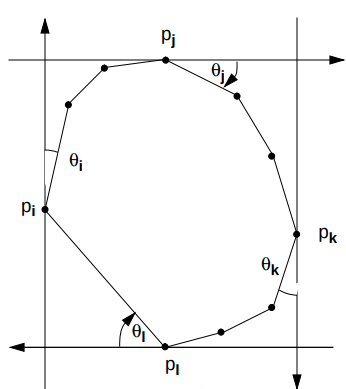
\includegraphics[width = 0.7 \linewidth]{pictures/rotating_calipers.png}
    \caption{Otáčející se třmeny}
    \label{fig:rotating_calipers}
\end{figure}

\section{Matematická morfologie}
\label{sec:morphology}
\todo[inline]{Popsání základních morfologických operací jako je dilatece, eroze, ...}

\section{RANSAC}
\label{sec:ransac}
\todo[inline]{popsání funkce ransac algoritmu}

\section{Vlastní čísla a vektory}
Pro čtvercovou matici \minsp{A}{R}{n\times n} a nenulový vektor \tl{v}\minsp{}{R}{n} a sklár $\lambda \in \mathbb{R}$ platí
\begin{align}
    \mathbf{Av} = \lambda \mathbf{v}.
\end{align}
Skalár $\lambda$ se nazývá vlastní číslo matice \tl{A} a vektor \tl{v} vlastní vektor příslušný vlastnímu číslu $\lambda$.
Spektrální věta (viz. \cite{Werner2020}) říka: Je-li matice \tl{A} symetrická, pak má $n$ vlastních čísel, kde $n = \text{rank}\mathbf{A}$ a všechna vlastní čísla jsou reálná.
\todo[inline]{Bude upraveno podle toho, co bude potřeba na popsání funkce PCA, SVD a ortogonální projekce}


\section{Singulární rozklad}
\todo[inline]{Stručně posat singulární rozklad PCA a ortogonální projekci na podprostor}
Singulární SVD\footnote{Z anglického Singular Value Decomposition}rozklad umožní každou matici \tl{A} $\in$ \spc{R}{m \times n} rozložit jako
\begin{align}
    \mathbf{A} = \mathbf{USV}^T
\end{align}
kde matice \tl{S} je diagonální, matice \tl{U} je ortogonální a obsahje vlastní vektory matice \tl{AA}$^T$, obdobně je pak i matice \tl{V} ortogonální a je složena z vlastních vektorů matice \tl{A}$^T$\tl{A}

\section{Ortogonální projekce na podprostor}
\label{sec:projekce}

\section{Analýza hlavních komponent}
%Analýza hlavních komponent (PCA\footnote{Z anglického Principal Component Analysis}) 


\chapter{Kamera}

\section{Dírkový model kamery}
Kamera zobrazuje body euklidovského prostoru $\mathbb{E}^3$, které jsou popsány pomocí světových souřadnic na body v euklidovské ploše $\mathbb{E}^2$, která se nazývá obraz. Body obrazu se označují jako pixely. 

Nejjednodušším modelem kamery je model dírkový, který má optické centrum, neboli centrum projekce, v konečnu. Centrum projekce umístíme do počátku kartézského souřadného systému a budeme uvažovat plochu kolmou na osu $Z$ našeho souřadného systému, kterou nazveme obrazovou rovinou. Ta je popsána jediným parametrem a to ohniskovou vzdáleností $f$. V dírkovém modelu kamery se bod v prostoru \tl{p} = $(x,y,z)^T$ promítne na bod obrazu pomocí zobrazení
\begin{align}
    \begin{bmatrix} x \\ y \\ z \end{bmatrix} \mapsto \begin{bmatrix} \sfrac{fx}{z} \\ \sfrac{fx}{z} \end{bmatrix},
    \label{pinhole_eq}
\end{align}
což odpovídá bodu, kde přímka spojující centrum projekce a bod v prostoru, protne obrazovou rovinu (viz obrázek \ref{pinhole}). Ve vztahu \ref{pinhole_eq} jsme předpokládali, že počátek souřadného systému obrazu je v optickém středu. Konvencí však je za počátek souřadnic zvolit levý horní roh obrazu. K zápisu využijeme homogenních souřadnic a dostaneme následující rovnici \unsure{pro zobrazení z souřadného systému kamery do systému obrazu s počátkem v levém horním rohu obrazu}
\begin{align}
    \begin{bmatrix} x \\ y \\ z \\ 1 \end{bmatrix} \mapsto \begin{bmatrix} fx + zc_x \\ fy + zc_y \\ z \end{bmatrix} = \begin{bmatrix} f & 0 & c_x & 0 \\ 0 & f & c_y & 0 \\ 0 & 0 & 1 &0 \end{bmatrix} \begin{bmatrix} x \\ y \\ z \\ 1 \end{bmatrix},
    \label{eq:pinhole_homogenous}
\end{align}
kde jsme jako $c_x$ a $c_y$ označili souřadnice optického středu. Označíme-li obecný bod v prostoru, který je popsán v souřadném systému kamer, \tl{x}$_p$ a odpovídající bod v rovině obrazu \tl{x}, pak můžeme rovnici \ref{eq:pinhole_homogenous} přepsat jako
\begin{align}
    \mathbf{x} = \mathbf{K}[\mathbf{I}\; |\; 0 ]\mathbf{x}_p \quad \mathbf{K} = \begin{bmatrix} f & 0 & c_x  \\ 0 & f & c_y  \\ 0 & 0 & 1  \end{bmatrix}.
    \label{intrinstic}
\end{align}
Matice \tl{K} se nazýva matice vnitřních parametrů kamery.

Obecně je bod $\mathbf{x}$ v euklidovském prostoru popsán v jiném souřadném systému, než je ten se kterým je svázána kamera. Tento souřadný systém se nejčastěji nazývá světový. Přechod do souřadného systému kamery ze světového je možno popsat následovně 
\begin{align} 
    \mathbf{x}_p = \begin{bmatrix} \mathbf{R} & -\mathbf{R\tilde C} \\ 0 & 1 \end{bmatrix}
    \mathbf{x}.
    \label{eq:world_to_cam}
\end{align}
Jako $\tilde{\mathbf{C}}$ jsme označili počátek souřadného systému kamery vyjádřený v světových souřadnicích a \tl{R} rotaci světového souřadného systému vzhledem ke kameře. Dosadíme-li nyní rovnici \ref{intrinstic} do \ref{eq:world_to_cam} dostaneme vztah popisující transformaci bodu z světových souřadnic do souřadnic obrazu
\begin{align}
    \mathbf{x} = \mathbf{KR}[\mathbf{I} \; | \; - \mathbf{\tilde C} ]\mathbf{x}.
    \label{eq:world_to_img}
\end{align}
Parametry $\mathbf{\tilde C}$ a \tl{R} se souhrně nazývají vnější parametry kamery. 
\begin{figure}
    \centering
    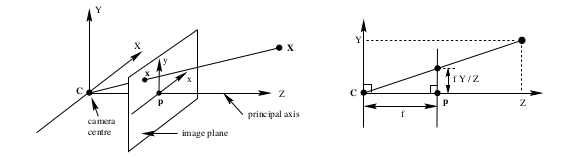
\includegraphics[width = 0.8\linewidth]{pictures/dirkovymodel_nakres.png}
    \caption{Model dírkové kamery}
    \label{pinhole}
\end{figure}

\section{Stereo kamera}
\subsection{Výpočet vzdálenosti}
Stereo kamera je tvořena dvěmi nezávislými čočkami. Zpracováním obrazů z obou čoček jsme schopni získat informace o hloubce každého pixelu. Budeme uvažovat model stereo kamery, kde jsou osy obou čoček rovnoběžné (viz obrázek \ref{stereo_paralel}). Osy jsou od sebe ve vzdálenosti $b$. Tomuto parametru se říka báze (baseline). Z podobnosti trojúhelníků plyne
\begin{align}
    \frac{z}{f} = \frac{x}{xl} \label{trojuh1} \\
    \frac{z}{f} = \frac{x - b}{xr} \label{trojuh2}.
\end{align}
Pokud z rovnice \ref{trojuh1} vyjádříme $x$ a dosadíme do rovnice \ref{trojuh2}, pak po úpravě dostaneme výsledný vztah pro vzdálenost bodu od kamery 
\begin{align}
    z = \frac{fb}{xl - xr} = \frac{fb}{d}.
    \label{depth_stero}
\end{align}
Hodnota $d$ se nazývá rozdíl (disparity) a $xl$, $xr$ jsou souřadnice bodu \tl{p} v levém, resp. pravém obrazu stereokamery. Pro každý bod v levém obrazu je tedy potřeba najít odpovídající bod v obrazu pravém (tzv. stereo pár). Bez jakékoliv apriorní znalosti by to znamenalo pro každý pixel prohledat celý druhý obraz, tedy náročnost hledání $\mathcal{O}(n^2)$. Pomocí epipolární geometrie můžeme hledání zúžit na přímku  a snížit tak náročnost hledání stereo páru na $\mathcal{O}(n)$. \cite{brown2003advances_in_stereo}

\subsection{Chyba výpočtu vzdálenosti}
Chyba výpočtu vzdálenosti se určí derivací rovnice \ref{depth_stero} podle $d$ \cite{keselman2017intel} 
\begin{align}
    \frac{\partial z}{\partial d} = \frac{z}{fb} \\
    |\epsilon_z | = \frac{z^2}{fb}|\epsilon_d |,
    \label{error_stereo}
\end{align}
kde $\epsilon_z $ je chyba určení vzdálenosti bodu a $ \epsilon_d $ je chyba rozdílu. toto je vlastnost kamery, popřípadě algoritmu použitého ke hledání odpovídajících párů, a nabývá téměř konstantních hodnot \cite{keselman2017intel}. Z rovnice \ref{error_stereo} tedy plyne, že chyba je úměrná kvadrátu vzdálenosti daného bodu a přesnost stereo kamer se vzdáleností rychle klesá.

\subsection{Epipolární geometrie}
\label{Sec:epipolar}
Epipolární geometrie se zabývá průnikem obrazových rovin se svazkem ploch, jejichž společná osa je báze. Uvažujme dvě dírkové kamery v obecném natočení, tedy jejich obrazové roviny nemusí být rovnoběžné, viz \ref{fig:epipolar}. Z dírkového modelu kamery plyne, že bod \tl{X}, který se nachází v euklidovském prostoru, a optické středy kamer $C, C'$ jsou koplanární a tvoří rovinu $p$. V místě, kde tato rovina protíná roviny obrazu, se nachází epipolární přímky \unsure{$l$ a $l'$ bold or normal text}. Hledáme-li stereo pár, pak pro známý bod \tl{x} (tj. projekce bodu \tl{X} do optické roviny levé kamery) musíme najít odpovídající bod \tl{x'}. Ten může ležet pouze na epipolární přímce $l'$, která je jednoznačně určena epipólem $e'$ a bodem $x'$. Epipól se nachází v místě, kde přímka spojující optická centra kamer protíná rovinu obrazu. Pro bod \tl{x'} platí
\begin{align}
    \mathbf{x'} = \mathbf{Hx},
\end{align}
kde \tl{H} je homografie mezi rovinami obrazu. Toto zobrazení je ovlivněno pouze vzájemnou polohou kamer a jejich vnitřními parametry. Nezávisí tedy na scéně.
Z bodu \tl{x'} se pak již lze určit epipolární přímku 
\begin{align}
    \mathbf{l'} = \mathbf{e'} \times \mathbf{x'} \\
    \mathbf{l'} = \mathbf{e'} \times \mathbf{Hx} \\
    \mathbf{l'} = \mathbf{Fx}.
\end{align}    
Matice \tl{F} se nazývá fundamentální a představuje zobrazení $f:\mathbb{R}^3 \mapsto \mathbb{R}^3$. Jelikož však platí $\text{rank} F = 2$, pak $\dim (\text{ker} F) = 1$
    Pokud jsou obě optické osy stereo kamery rovnoběžné, pak se výpočet epipolární přímky velice zjednodušší, jelikož homografie mezi rovinami obrazu je pouze posunem ve směru báze.
\begin{figure}

    \centering
    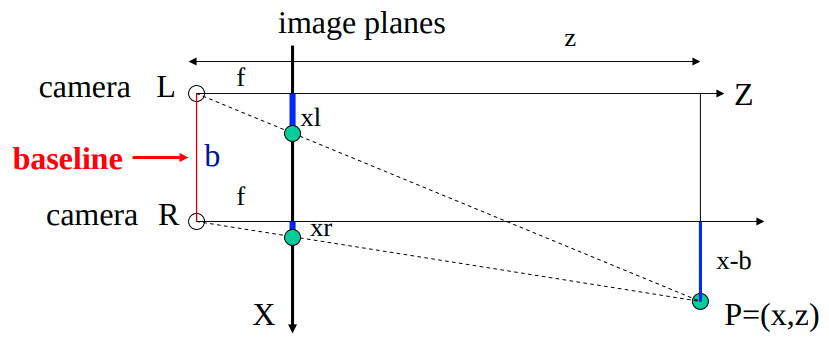
\includegraphics[width = 0.8\linewidth]{pictures/stereo_sketch.png}
    \caption{\cite{washingtion_steropic}}
    \label{stereo_paralel}
\end{figure}
\section{Hledání stereo páru}
Metody užívané pro hledání stereo páru se dělí na metody plošné (area based) a metody založené na porovnávání rysů (features). Při hledání stereo páru se často využívá následujících omezení, která tento proces zjednodušší. Tato omezení však v extrémních případech, jako je například okluze,  nemusí platit.
\begin{itemize}
    \item Epipolární omezení: Pixel v druhém obrazu se nachází ( pokud existuje ) na epipolární přímce ,viz. sekce \ref{Sec:epipolar}.
    \item Spojitost: Rozdílová, popř. hloubková, mapa by měla být po částech spojitá.
    \item Jedinečnost: Každý pixel v levém obrazu má k sobě právě jeden odpovídající v obrazu pravém. 
    \item Pořadí: Pořadí pixelů v levém obrazu odpovídá pořadí v pravém.
\end{itemize}

\subsection{Plošné metody}
Využívají informaci z okolí pixelu. Ty jsou porovnány se všemi přípustnými pozicemi v druhém obrazu a bod, jehož hodnota je nejblíže vzoru, tvoří stereo pár. Mezi nejpoužívanější variace plošných metod patří následující.

\subsubsection{Součet absolutních rozdílů}
Je definována konstatní velikost okolí pixelu $\mathbf{x}(u,v)$. Následně jsou hodnoty všech pixelů v okně sečteny a výsledná hodnota je provnána s body v pravém obrazu, kde se může korespondující pixel nacházet, tj. body které splnují námi používaná omezení. Pro odpovídající bod \tl{x'} tedy platí
\begin{align}
    \mathbf{x'} = \text{argmin}\left( \displaystyle\sum_i \displaystyle\sum_j |\mathbf{I}_l(u+i,v+j) - \mathbf{I}_r(u+i, v+j + d)| \right),
\end{align}
kde $\mathbf{I}(u,v)$ je intenzita příslušného pixelu, $d$ je posun okna ve druhém obrazu a součet probíha přes celé okno. Vztah byl zjednodušen uvažováním horizontálních epipolárních přímek. Toto odpovídá konfiguraci kamery s rovnoběžnými optickými osami.

    Existuje mnoho podobných algoritmů, které se liší pouze metrickou funkcí. Místo absolutní hodnoty rozdílu je užit například kvadrát rozdílu  nebo jeho normalizovaný kvadrát. Jedná se o nejrychlejší algoritmy pro hledání stereo páru, přesto však dosahují vysokých přesností \cite{kuhl2005comparison}. 

\subsubsection{Cenzus}
\label{Sec:cenzus}
Jedná se o variaci algoritmu patřící do rodiny plošných metod, které před porovnáním hodnot pixelů provedou určitou transformaci obou obrazů. Patří sem naříklad i transformace podle hodnoty (rank transform). Cenzus opět pracuje se definovanou maskou kolem pixelu, pro který hledá stero pár. Pixely, které se nachází v šabloně, se transformují na vektor jedniček a nul podle toho, zda je hodnota intenzity pixelů masky větší, popřípadě menší, než intenzita centrálního pixelu. Stejná transformace se provede i v pravém obrazu pro každý pixel, který může doplnit stereo pár. Vektory jsou následně porovnány a je vybrán ten, jehož vektor má nejmenší Hammingovu vzdálenost. \cite{kuhl2005comparison, brown2003advances_in_stereo}

\subsection{Porovnávání rysů}
Pro každý obraz jsou vygenerovány důležité body. To mohou být například hrany či rohy v obrazu. Tyto rysy jsou porovnány s analogicky vygenerovánými rysy v druhém obrazu. Tento postup se v některých aplikacích opakuje, přičemž v každém dalším kroku je každý rys rozložen na několik menších, o kterých již máme apriorní znalost jejich přibližné polohy. Aby bylo možné sestavit obraz pouze z několika rysů, je nutné provést časově náročné předzpracování obrazu za ůčelem najití vhodných rysů a po nalezení korespondujících rysů provést zpětnou rekonstrukci obrazu. \cite{brown2003advances_in_stereo}

%\todo[inline]{dolnit }
Pro porovnání rysů mezi levým a pravým obrazem se využívá algoritmů jako je například SIFT (Scale Invariant Feature Transform), SURF (Seeded-Up Robust Features) nebo BRIEF(Binary Robust Independent Elementary Features).

\begin{figure}
    \centering
    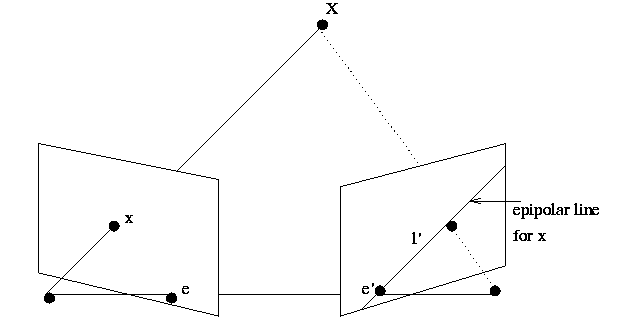
\includegraphics[width = 0.8\linewidth]{pictures/epipolar.png}
    \caption{Placeholder}
    \label{fig:epipolar}
\end{figure}
%TODO uncoment this ( avoiding compilation warnings )




%\section{Intel \textregistered Realsense\textsuperscript{TM} D435}
\section{Intel Realsense D435}
Intel\textregistered{} Realsense\textsuperscript{TM} D435 je širokoúhlá stereo kamera, která se skládá z RGB kamery, infračerveného projektoru a dvou infračervených kamer, jejichž data jsou zpracovává přímo v čipu kamery dedikovaným procesorem. Výstupem z kamery je tedy barevný obraz (RGB) a vzdálenost jednotlivých pixelů neboli hloubková mapa. 

\begin{figure}
    \centering
    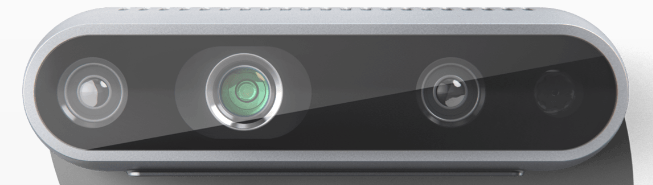
\includegraphics[width = 0.8\linewidth]{pictures/realsense_kamera.png}
    \caption{Fotografie kamery Intel\textregistered{} Realsense\textsuperscript{TM} D435 \cite{Realsense_obrazek}}
    \label{Fig:realsense_pic}
\end{figure}

    Dvě infračervené kamery jsou v konfiguraci s rovnoběžnými optickými osami ve vzdálenosti 50$\,mm$. Infračervený projektor promítá na scénu statický obrazec, který se nachází mimo viditelné spektrum a není tedy zachycen RGB kamerou. Tento obrazec slouží k najítí stereo párů, zejména pak u objektů s řídkou texturou.

    Kamera je vybavena specializovaným procsorem Vision Processor D4 pro výpočet hloubkové mapy. Ten je schopen při rozlišení hloubkové kamery 848x480 zpracovávat až 90 snímků za sekundu (FPS). Při této rychlosti snímání je přesnost kamery výrazně snížena \cite{keselman2017intel}. Pro maximální přesnost je vhodné nastavit frekvenci na 30 snímků za sekundu. 
    
    Procesor má stejně jako celá kamera velice nízký odběr elektrické energie. Celá kamera včetně IR projektoru má odběr menší než jeden watt a je tedy vhodná pro mobilní aplikace, kde je velikost baterie a spotřeba energie omezujícím faktorem. \cite{RealSense_datasheet} \todo[inline]{Porovnání s Kinectem a Asus RGBD kamerou}

    Pro hledání stereo párů je využit algoritmus cenzu popsaný v \ref{Sec:cenzus} s maskou o velikosti $7 \times 7 $. Výsledky jsou následně ověřovány sadou filtrů, které měří důvěryhodnost shody. Podle nastaveného limitu důležitosti pak pro tento pixel buď vygenerují záznam v hloubkové mapě, nebo pixel zůstane nevyplněn. Výsledky kamery pro různé hodnoty limitu jsou vidět v tabulce \ref{fig:tablka_limity}. 
\begin{figure}
    \centering
    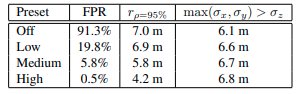
\includegraphics[width = 0.8\linewidth]{pictures/realsense_threshold.png}
    \caption{Postupně zleva: Hodnota limitu, počet falešných shod pokud je scéna blíže než je minimální vzdálenost detekce kamerou. Vzdálenost, kdy vyplněnost hloubkové mapy klesne pod $95\%$, a vzdálenost při které je směrodatná odchylka ve směru osy $z$ menší než ve směru $x$ a $y$ \cite{keselman2017intel}}
    \label{fig:tablka_limity}
\end{figure}

Procesor kamery není schopen určit hloubku bodů, pokud se objekt nachází příliš blízko. Konkrétní hodnoty je možno vidět v tabulce \ref{fig:minimalni_hloubka}. Maximální měřitelná vzdálenost je za ideálních podmínek až 40 metrů \cite{keselman2017intel}. S rostoucí vzdáleností se kamera chová podle rovnice \ref{error_stereo} a přesnost tedy rychle klesá. Toto chování neodpovídá rovnici \ref{error_stereo}, pokud kamera operuje s objekty, které se nachází na obou hranicích měřitelné vzdálenosti. Ilustrace výstupu kamery, pokud se objekt nachází ve vzdálenosti meší než specifikuje tabulka \ref{fig:minimalni_hloubka} je vidět na obrázku \ref{fig:rs_bad}.

\begin{figure}
    \centering
    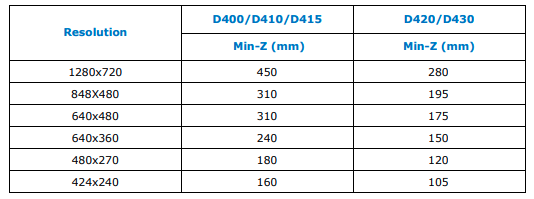
\includegraphics[width = 0.8\linewidth]{pictures/minimalni_vzdalenost.png}
    \caption{Tabulka minimální detekovatelné hloubky \cite{RealSense_datasheet}}
    \label{fig:minimalni_hloubka}
\end{figure}

\begin{figure}
\centering
\begin{subfigure}{0.48\textwidth}
  \centering
  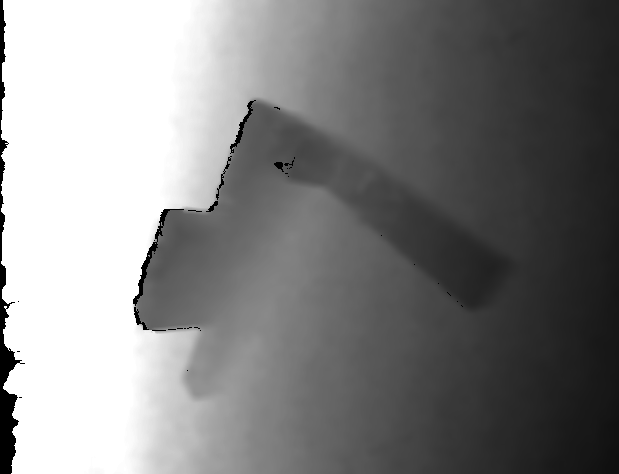
\includegraphics[width=0.9\linewidth]{pictures/good_realsense.png}
  \caption{Snímek bez výrazných výpadků dat hloubkové mapy}
  \label{fig:rs_good}
\end{subfigure}
\begin{subfigure}{0.49\textwidth}
  \centering
  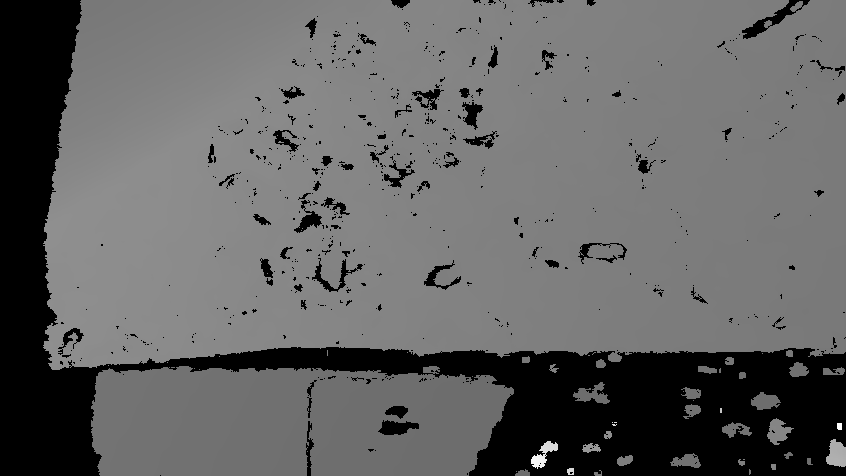
\includegraphics[width=0.9\linewidth]{pictures/bad_realsense.png}
  \caption{Snímek s chybějícími hloubkovými daty}
  \label{fig:rs_bad}
\end{subfigure}
\caption{Výstupní data kamery Realsense, hloubková data byla převedena do odstínů šedé}
\label{fig:realsense_pics}
\end{figure}

\section{Metody v detekci objektů z hloubkových dat}
\label{sec:Metody_detekce}
Existuje spoustu různých metod pro detekci objektů z hloubkových dat. Ty se liší podle různorodosti detekovaných objektů, požadavků na čas výpočtu, možnosti získání trénovacích dat nebo formátem vstupních dat. Obvyklým formátem je mračno bodů, neboli point cloud, což je nestrukturovaná množina bodů v trojrozměrném prostoru. Zejména v posledních letech s nástupem hloubkových kamer jako je například Microsoft Kinect, Asus Xtion nebo námi používaný Intel RealSense, se čím dál více používájí data ve formátu RGB-D obrazu. Ten se dá pomocí vztahu \ref{eq:pinhole_homogenous} převést na point cloud. Výstupní data z hloubkové kamery bývají většinou oproti LIDARu méně přesné. Výhodou naopak je vysoká vzorkovací frekvence, velké množství výstupních bodů a cena.
\subsection{Klasické metody}

\subsubsection{Určení normálového vektoru plochy z nestrukturovaných dat}
\label{subsec:nomrmal_est}
Téměř všehny metody detekce z objektů se skládájí z více kroků a jedním z nich většinou bývá určení normálového vektoru plochy. Obvykle se jedná o plochu reprezentující zem, popřípadě jinou podložku, nebo plochy reprezentující stěny místnosti. Přístupy k hledání ploch v obrazu se výrazně liší, uvedeme příklady některých z nich.

\begin{itemize} 
    \item Použití hrubé síly (brute force). Postupně jsou vyzkoušeny všechny možnosti, popřípadě část z nich, a vybere se nejlépe vyhovující. Využívá se zde zejména algoritmů jako je RANSAC, případně jeho modifikace. Tato metoda je vhodná zejména pokud jsou data zatížena silným šumem, jelikož při správném počtu iterací téměř vždy vrátí správný výsledek. Toto je však vykoupeno vysokou časovou náročností \cite{RANSAC_plane,single_RGBD_reconstruction}, která se dá snížit vhodný předzpracováním dat, například segmentací na menší celky a určením plochy pouze pro tyto segmenty. \cite{rusu2009close}
    \item Výpočet normálového vektoru v každém bodě. Normálový vektor je kolmý na plochu reprezentující okolí bodu. Toto okolí je tvořeno body nacházejícími se v okruhu o poloměru $r$ \cite{wang2015dominant} ,popřípadě $k$ nejbližšími body\cite{holz2011real,trevor2013efficient}. Poté je provedena segmentace pomocí metody rostoucích oblastí viz. sekce \ref{subsection:segmentation}. Výstupem jsou tedy skupiny bodů, které představují jednotlivé plochy. V některých případech je navíc použit RANSAC na již nalezené segmenty za účelem vyloučení bodů, které leží mimo plochu představovanou daným segmentem, přestože jejich normálový vektor dané ploše odpovídá \cite{lai2011large}.
    \item Jsou nalezeny body, které patří do dané roviny, a těmi je poté pomocí PCA proložena rovina \cite{zhang2016fast}. Tato metoda vyžaduje přesné určení bodů, o kterých se předpokládá, že tvoří danou rovinu. Jediný bod ležící ve velké vzdálenosti od roviny (outlier) může způsobit velké nepřesnosti, jelikož rovina je proložena body metodou nejměnších čtverců.
\end{itemize}

%\subsubsection{ Použití hrubé síly (brute force)} Postupně jsou vyzkoušeny všechny možnosti, popřípadě část z nich a vybere se nejlépe vyhovující. Vužívá se zde zejména algoritmů jako je RANSAC, popřípadě jeho modifikace. Tato metoda je vhodná zejména pokud jsou data zatížena silným šumem, jelikož při správném počtu iterací téměř vždy vrátí správný výsledek, toto je však vykoupeno vysokou časovou náročností.\cite{RANSAC_plane,single_RGBD_reconstruction} Tato se dá snížit vhodný předzpracováním dat. Například segmentací na menší celky a určením plochy pouze pro tyto segmenty \cite{rusu2009close}
%\subsubsection{Výpočet normálového vektoru v každém bodě}, kde je normálový vektor kolmý na plochu reprezentující okolí bodu, toto je tvořeno body nacházejícími se v okruhu o poloměru $r$ \cite{wang2015dominant} popřípadě $k$  nejbližšími body\cite{holz2011real,trevor2013efficient}. Poté je provedena segmentace pomocí metody rostoucích oblastí viz. sekce \ref{subsection:segmentation}. Výstupem jsou tedy skupiny bodů, které reprezentují jednotlivé plochy. V některých případech je ještě použit RANSAC na již nalezené segmenty, aby byly vyloučeny body, které leží mimo plochu přesto, že jejich normálový vektor dané ploše odpovídá \cite{lai2011large}.
    %Jsou nalezeny body, které patří do dané roviny, těmito je poté pomocí PCA proložena rovina \cite{zhang2016fast}. Tato metoda je náchylná na body ležící mimo rovinu (outliers), jelikož rovina je proložena body ve smyslu nejměnších čtverců a jediný bod ležící ve velké vzdálenosti od roviny může způsobit velké nepřesnosti.

\subsection{Segmentace obrazu}
\label{subsection:segmentation}
Důležitým krokem pro porozumění obrazu a detekci objektů je segmentace obrazu, tj. rozdělení vstupních dat na skupiny. Rozdělujeme dva typy segmentace. Sémantickou, která sjednocuje body reprezentující danou skupinu objektů (např. všechny bloky ležící na zemi), a segmentaci jednotlivých instancí, kdy je skupina objektů rozdělena na jednotlivé zástupce dané skupiny. 

    Přístup k segmentaci se líší podle dané aplikce. Nejpoužívanějšími metodami jsou tyto:
\begin{itemize}
    \item Metoda prahování. Body $\mathbf{p}(x,y)$ jsou rozděleny do $m$ skupin podle toho, zda jejich vlastnost $V$, což je například vzdálenost bodu od kamery nebo od plochy, dosahuje stanovené hodnoty $T_m$. Tato hodnota může být pevně určená, nebo se může dynamicky měnit, a to v závislosti na okolních bodech, nebo v závislosti na pozici v obrazu, tj. $T(x,y)$. Pro prahovací metodu tedy platí následující vztah
        \begin{align}
\left\{ 
        \begin{gathered}
            \mathbf{p} \in m \text{ iff } V(\mathbf{p}) > T_m \\
            \mathbf{p} \in n \text{ iff } V(\mathbf{p}) > T_n \\
            \mathbf{p} \in \emptyset \text{ iff } V(\mathbf{p}) \leq T_1 
        \end{gathered}
\right\}.
        \end{align}
 
    \item Metoda detekce hran. V obrazu jsou detekovány prudké změny pozorované vlastnosti $V$ v bodě \tl{p} za pomoci první derivace vlastnosti $V$ v bodě \tl{p}. Pokud hodnota derivace dosáhne daného prahu je \tl{p} registrován jako hrana. Po výpočtu bývá provedena úprava těchto hran, kterou je například filtrování, popřípadě spojení některých sousedních bodů. Nakonec jsou v obrazu identifikovány segmenty bodů, které jsou od zbytku odděleny hranou. K určení hran se využívá například Sobelova operátoru, který byl popsán v sekci \ref{subsec:sobel}, nebo Cannyho operátoru.

    \item Metoda rostoucí oblasti. Ta se dělí na dva typy: S počátečním bodem (seed) a bez počátečního bodu. 

    Je zvolen jeden, popřípadě několik počátečního bodů. K těmto se postupně přidávají sousední body, pokud splňují předem definované podmínky. Těmi jsou například maximální odchylka normálových vektorů bodů od normálového vektoru seedu, nebo rozdíl velikost některé souřadnice. Metoda bez počátečního bodu pak rozdělí všechny body do skupin, jejichž body spolu sousedí a zároveň mají podobné vlastnoti. Jedná se o algoritmus, který pracuje s konstatní časovou náročností odpovídájící $\mathcal{O} (2n)$, kde $n$ je počet pixelů obrazu. 

\item Metoda rozdělovaní a slučování. Obraz je postupně rozdělen na části, které mají podobnou charakteristiku. Následně jsou sousední regiony, které jsou si podobné, sloučeny do jedoho. Pro reprezentaci regionů se obvykle využívá kvadrantový strom (quadtree).

    Nechť $o$ je obraz a $V$ daná vlastnost jednotlivého bodu \tl{p}. Skupina bodů má vlastnost $V$, pokud tuto vlastnost má každý bod skupiny. Metodu rozdělování a slučování lze za těchto podmínek popsat následovně.\cite{segmentace_metody}
    \begin{itemize}
        \item Region $R_1$ je roven $o$.
        \item Pokud platí $V(R_i) = False$, pak je region rezdělen na několik menších.
        \item Pokud platí $V(R_i) = True$, pak je $R_i$ sloučen se všemi sousedními regiony $R_j$, přičemž musí platit $V(R_i \cup R_j)$. Tento krok se opakuje, dokud je možné některý region sloučit.
    \end{itemize}         %jsou body s podobným normálovým vektorem spojeny do větších regionů a tyto reprezentují jednotlivé plochy, k tomuto se využívá různých modifikací CCA (Connected Component Analysis) algoritmu, tento existuje v následujících dvou konfiguracích. S počátečním bodem (seed), kdy je určen jeden bod (popřípadě nekolik boudů), ke kterému se postupně přidávají sousední body, pokud jejich normálový vektor má maximálně předem definouvanou odchylku a normálového vektoru seedu. Bez počátečního bodu, jedná se o algoritmus, který pracuje s konstatní časovou náročností, která odpovídá $\mathcal{O} (2n)$, kde $n$ je počet pixelů obrazu
\item Metoda shlukování (clustering). Obraz je rozdělen do shluků, ve kterém má každý bod podobné vlastnosti, resp. jejich vlastnosti jsou si v rámci obrazu nejbližší. Vlastnost v tomto případě bývá nejčastěji euklidovská vzdálenost. Mezi nejpopulárnější algoritmy patří\footnote{Princip algoritmů bude vysvětlen při shlukování podle euklidovské vzdálenosti}
    \begin{itemize}
        \item K-means algoritmus. V tomto algoritmu je předem nutné znát počet shluků $m$, do kterých budou body rozděleny. Následně se náhodně vybere $m$ bodů, které představují střed shluku. Poté je pro každý bod spočítána vzdálenost od jednotlivých středů. Bod je přiřazen do daného shluku, jehož vzdálenost středu je nejmenší. Následuje přepočítaní středů a postup se opakuje. Ve chvíli kdy již nedochází ke změnám mezi jednotlivými shluky je zaznamenán součet rozptylů bodů v rámci jednotlivých shluků a celý proces počínaje náhodnou volbou středů se $n$-krát opakuje. Nakonec je vybrán výsledek, který má nejmenší rozptyl.
        \item Mean-shift algoritmus. Je předem definován poloměr kruhového okna $r$. Následně je náhodně určeno (popřípadě podle předem definované masky rozmístěno) $n$ bodů \tl{p}. V každé iteraci se spočítá střed bodů $\mathbf{t}$, pro které platí $||\mathbf{t} - \mathbf{p}|| < r$, ty naradí bod \tl{p}. Tento postup se opakuje, dokud body konvergují. Výsledná poloha bodů $\mathbf{p}_i$ pak představuje sřed jednotlivých shluků. 
        \item DBSCAN (Density-Based Spatial Clustering of Applications with Noise) algoritmus. Všechny body obrazu jsou označeny jako nenavštívené. Náhodně je vybrán nenavštívený bod \tl{a} a pokud se v jeho okolí o velikosti $\epsilon$ nachází minimální předem zvolený počet bodů, je celé okolí bodu \tl{p} přidáno do shluku a postup se opakuje pro přidané body. Pokud již nelze žadný další bod přidat zvolí se další nenavštívený bod a proces se opakuje pro další shluk. Toto probíhá dokud existují nenavštívené body. 
    \end{itemize}
\end{itemize}

\subsubsection{Detekce objektů}

\subsection{Metody na bázi neuronových sítí}
\todo[inline]{Již daleko stručněji porovnat klasické metody s těmi, které využívají CNN. Popsat výhody a nevýhody oproti klasickým metodám}


\section{Navržené řešení}

Navržené řešení se skládá ze 3 částí a to v souladu se sekcí \ref{sec:Metody_detekce}, tedy nalezení normálového vektoru podložky, segmentace obrazu na jednotlivé cihly a následné nalezení ohraničujících boxů pro jednotlivé cihly. Pro všechny části řešení bylo navrhnuto více postupů a jejich výsledky jsou porovnány v sekci \ref{sec:závěr}. Ve všech částech se vychazí ze zadání, které specifikuje, že na zemi nemůže být kromě cihel žadný jiný objekt podobných rozměrů. Velikost cihel je předem známa, mimo jejich délky, která může nabývat různých rozměrů. Cihly na sebe mohou být naskládany v libovolném počtu vrstev, mohou se objevit v libovolném natočení a navzájem se dotýkat. dále platí, že pokud se nachází některá cihle v patře $n$, tak ve všech patrech $0,...,n-1$ se pod touto cihlou také nachází cihly. To znemená, že pokud jsou cihly postaveny do zdi, pak tato zeď nemá díry.

V některých částech byl zaveden předpodklad doteku dvou cihel pouze po celé délce odpovídajících stěn za účelem rychlejší alternativy detekce.
\subsection{Detekce normálového vektoru a sémantická segmentace obrazu}
\label{sec:normal_est}
\subsubsection{Přístup založený na výšce}
\label{subsec:height}
Začneme určením normálového vektoru roviny reprezentující zem. Z jeho znalosti, můžeme odečtením plochy představující zem, najít body ležící nad zemí, tj. body představující cihly. Dostaneme tedy sémanticky segmentovaný obraz.

Vytvoříme mřížku bodů, které jsou v místech, kde předpokládáme přesný výstup kamery. U těch ověříme, zda pro ně byla kamerou vygenerována hloubka a zda bod leží v maximální vzdálenosti 4\,$m$, jelikož podle \cite{keselman2017intel}  chyba stereo kamery RealSense D435 nad tuto vdálenost začíná být markantní a správné určení normálového vektoru je zásadní pro všechny ostatní kroky. Množinu bodů $M = \mathbf{a}_1 \dotsc \mathbf{a}_m$, které splňují výše uvedená kritéria, proložíme rovinou pomocí PCA algoritmu a dostaneme normálový vektor \tl{n} plochy $p$ minimalizující kvadrát vzdáleností od bodů. Tato plocha je posunuta mimo počátek o $d$.
\begin{align}
    \mathbf{\bar{a}} = \frac{1}{m}\left( \mathbf{a}_1 \dotsc \mathbf{a}_m \right) \\
    d = \mathbf{n} \cdot \mathbf{\bar{a}} = \mathbf{n}^T \mathbf{\bar{a}} \\
    p: n_1x + n_2y + n_3z - d = 0 \label{normal_plane}
\end{align}
Každý bod \tl{a} je buď součástí země, nebo součastí cihly. Je-li v množině $M$ $k$ bodů, které jsou součastí země $G$, pak zbylých $m - k$ bodů musí být součastí mračna bodů reprezentující cihlu $C$. Tyto body se vždy nachází ve výšce $z$ \footnote{Osa z směřuje směrem z kamery a body nacházající se nad zemí mají tedy menší hodnotu $z$.}nad zemí a tedy pro každý bod \tl{a} platí
\begin{align}
    n_1a_1 + n_2a_2 + n_3a_3 + \epsilon > d \; \rightarrow \; \mathbf{a} \in C  \\
    n_1a_1 + n_2a_2 + n_3a_3 + \epsilon \leq d \; \rightarrow \; \mathbf{a} \in G,
\end{align}
kde $\epsilon$ je experimentálně určená hodnota ošetřující případy, kde $k = m$, tj. všechny body reprezentují zem. V tomto případě čast bodů bude ležet nad plochou $p$. To jest dáno šumem dat a nepřesností kamery. Přidáním parametru $\epsilon$ je zajištěno, že každý bod reprezentující zem bude správně klasifikován i při zašuměných datech.

Po výběru bodů z mřížky podle výše uvedených kriterií dostaneme $k$ bodů, které reprezentují zem a nacházejí se v místech, kde je přesnost kamery v rámci jejich možností nejvyšší. Tyto body by se daly znovu proložit plocho, čímž bychom dostali aproximaci natočení země pomocí normálového vektoru \tl{n}. Vzhledem k důležitosti přesnosti určení \tl{n} získáme další body reprezentující zem pomocí algoritmu \ref{alg:floodfill}. Tyto body opět pomocí PCA proložíme rovinou a dostaneme přesnější aproximaci normálového vektoru země, viz. sekce \ref{sec:závěr}. Na obrázku \ref{fig:floodfill} lze pozorovat výsledek algoritmu \ref{alg:floodfill}.\unsure{musí být algoritmus v české jazyce? Zejména pak notoricky známé pojmy jako stack atd... }
    
    
\begin{algorithm}
    \caption{Expandování bodů }
    \label{alg:floodfill}
    \begin{algorithmic}
        %\STATE S = stack
        %\STATE G = points that belongs to ground
        %\STATE V = visited points
        \STATE $Stack \gets \emptyset$
        \STATE $G \gets \emptyset$
        %\STATE $V \gets \emptyset$ \quad //visited points
        \FOR{$\mathbf{a}$ in $M$}
            \STATE Stack.push($\mathbf(a)$)
            \STATE $z \gets$ height of $\mathbf{a}$
            \WHILE{\NOT Stack.empt()}
                \STATE $\mathbf{t} \gets$ Stack.pop()
                \STATE $G \gets G \cup t$
                \STATE $V \gets V \cup p$
                \FOR{$\mathbf{n}$ in neighbours of $\mathbf{t}$}
                    \STATE $zn \gets$ height of $\mathbf{n}$
                    %\IF{$zn \in \left[ z - \delta , z + \delta\right]$ \AND \NOT $\mathbf{n}$ $\in V$}
                    \IF{$zn \in \left[ z - \delta , z + \delta\right]$ \AND \NOT $\mathbf{n}$ $\in G$}
                    \STATE stack.push($\mathbf{n}$)
                    \ENDIF
                \ENDFOR
            \ENDWHILE
        \ENDFOR
    \end{algorithmic}
\end{algorithm}

\begin{figure}
    \centering
    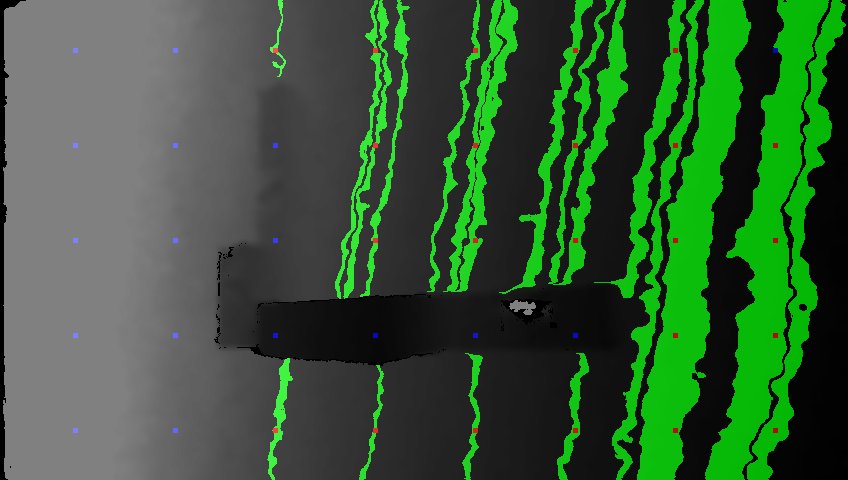
\includegraphics[width = \linewidth]{pictures/prob0001body_gnd.png}
    \caption{Červenou barvou jsou znázorněny body, ze kterých probíhal algoritmus \ref{alg:floodfill}, modré body byly podle výše uvedených kritérií vyřazeny a zeleně jsou znázorněny výsledné body reprezentující zem}
    \label{fig:floodfill}
\end{figure}

Nyní vypočítáme výšku každého bodu nad rovinou a podle této vzdálenosti přidělíme hodnotu 0 až $k$, kde číslo reprezentuje očekávaný počet na sobě naskládaných cihel a $k$ maximální počet cihel, jež může být na sebe naskládán. Vizualizace tohoto výsledku je vidět na obrázku \ref{fig:height_map}

\begin{figure}
    \centering
    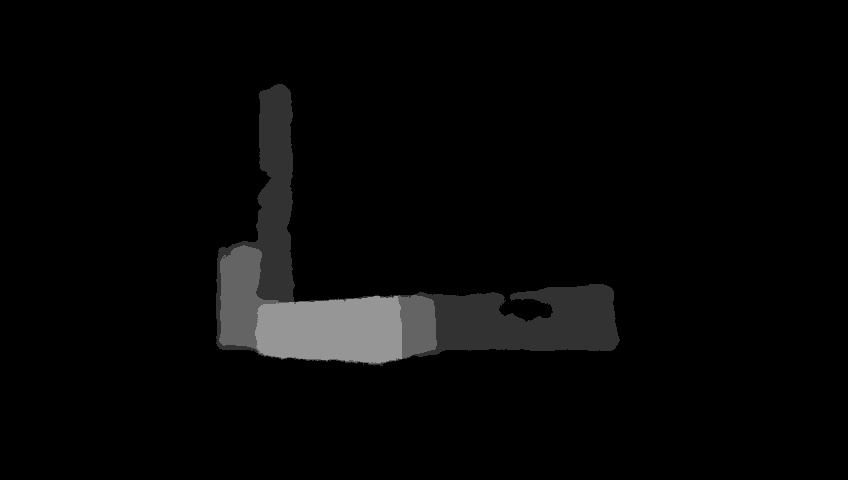
\includegraphics[width = \linewidth]{pictures/original_vrstva2_pic1.jpg}
    \caption{Vzdálenost boudů od roviny zobrazena jako počet na sobě lžících cihel}
    \label{fig:height_map}
\end{figure}

\subsubsection{Detekce normálového vektoru pomocí RANSAC}
Body jsou postupně prokládány roviny pomicí RANSAC algoritmu, viz. \ref{sec:ransac}. Zde je potřeba správně určit kritérium, při jehož splnění budeme mít jistotu, že dotekovaaná plocha představuje zem. Pokud by algoritmus skončil po detekci plochy, v jejimž okolí leží nejvíce bodů. Mohli bychom při velkém zastoupení kostek v obrazu dostat rovinu popisující horní stěnu těchto kostek. Jako terminační kritérium je tedy zvolena detekce dvou rovin a jejich následným porovnáním vybereme tu, která popisuje zemi.

\subsubsection{Přístup založený na změně výšky}
Velice populární postup při segmentaci obrazu je založen na porovnání normálového vektoru v bodech obrazu. Normálový vektor je vypočten pro každý bod obrazu a následně jsou body, jejichž normálový vektor má podobný směr, popřípadě i velikost, sloučeny do větších celků. V našem případě je vrchní stěna cihly paralelní se zemí a má tedy stejný normálový vektor. Nachází se však v jiné výšce. Pomocí výpočtu gradientu, který budeme realizovat užitím Sobelova operátoru aplikovaného na výšku bodů, spočítáme derivaci výšky. Ta by měla být nejvyšší v oblasti přechodu země - cihla. Následně pak sloučíme body s hodnotou gradientu výšky, která se liší v rámci skupiny maximálně o $\delta$. K tomu bylo využito upraveného CCL (Connected-component labeling) algoritmu. 

Tato metoda při správném odladění parametru $\delta$ funguje velice přesně. Problémem je však robustnost. Hodnoty parametru $\delta$ fungující na cihly v blízkosti kamery nedetekují cihly ve vzdálenosti řadově 2\,$m$ a více a naopak. Toto je způsobeno jednak šumem kamery, který podle rovnice \ref{error_stereo} roste kvadraticky, a zejména pak zkreslením vzdálenější hrany cihly kamerou, viz. obrázek \ref{fig:point_cloud_grad}. Kamera zde špatně nachází stereo páry a generuje mračna bodů, která ve skutečnosti neexistují. Ty zmírňují přechod cihla-zem a snižují tak hodnotu gradientu. Toto chování je dobře vidět na obrázku \ref{fig:sobel_segment}.
\begin{figure}
    \centering
    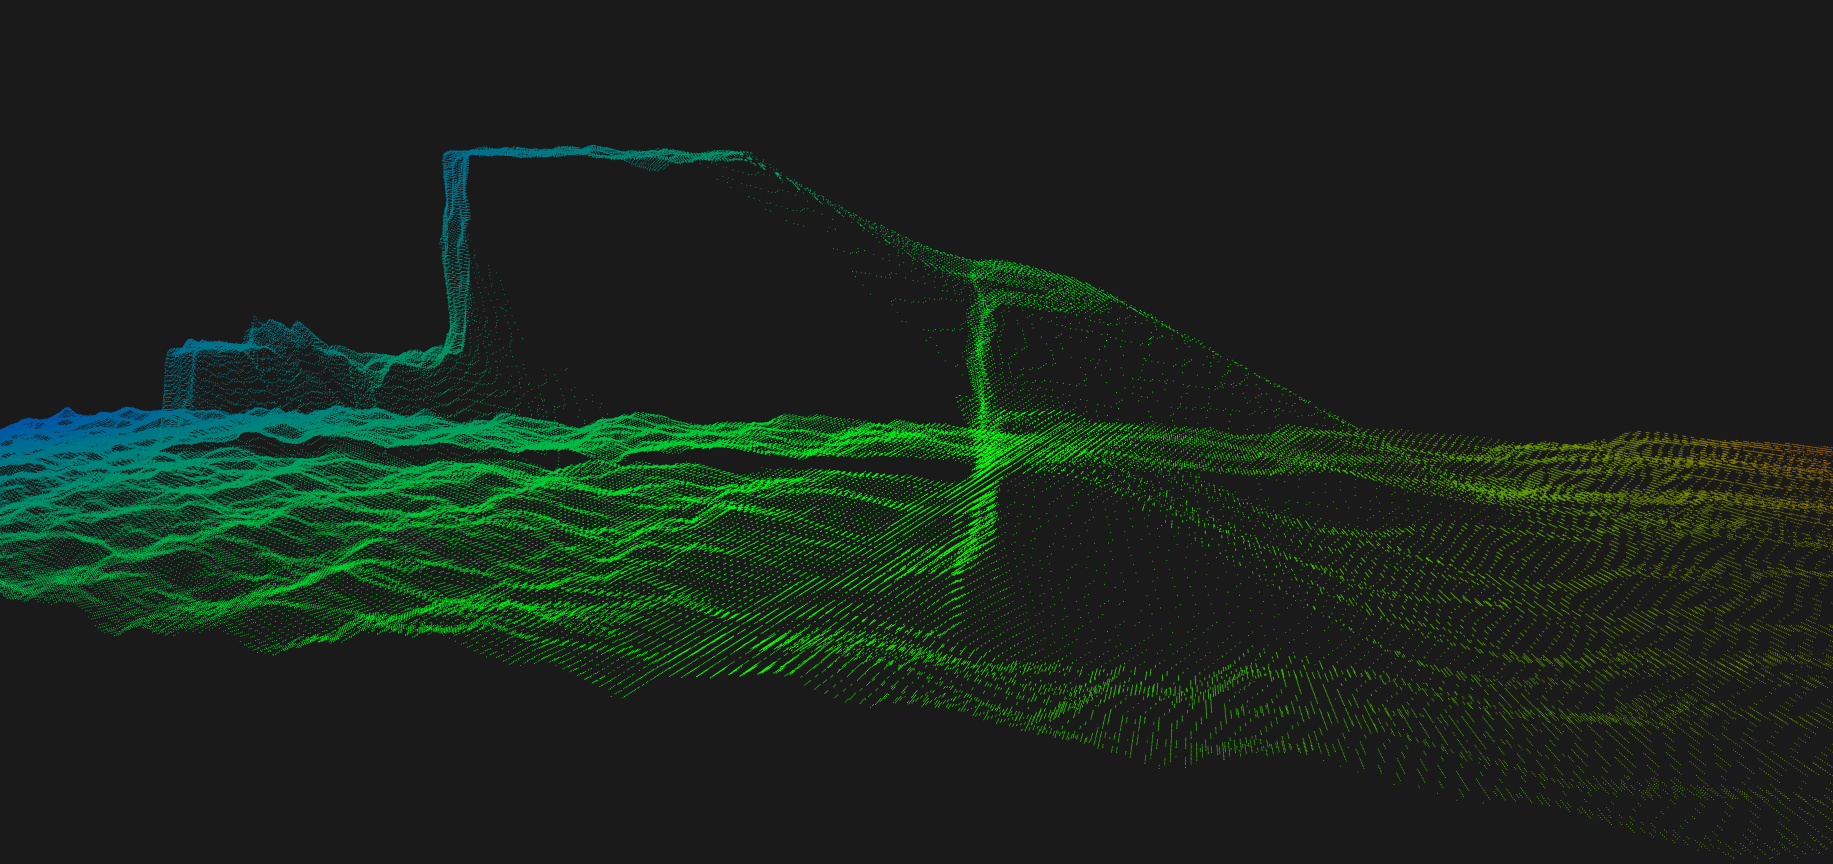
\includegraphics[width = \linewidth]{pictures/pc_crop.png}
    \caption{Výstup kamery - mračno bodů zobrazující skupinu cihel. V pravé části je vidět zkreslení hrany způsobující problém při segmentaci}
    \label{fig:point_cloud_grad}
\end{figure}

\begin{figure}
    \centering
    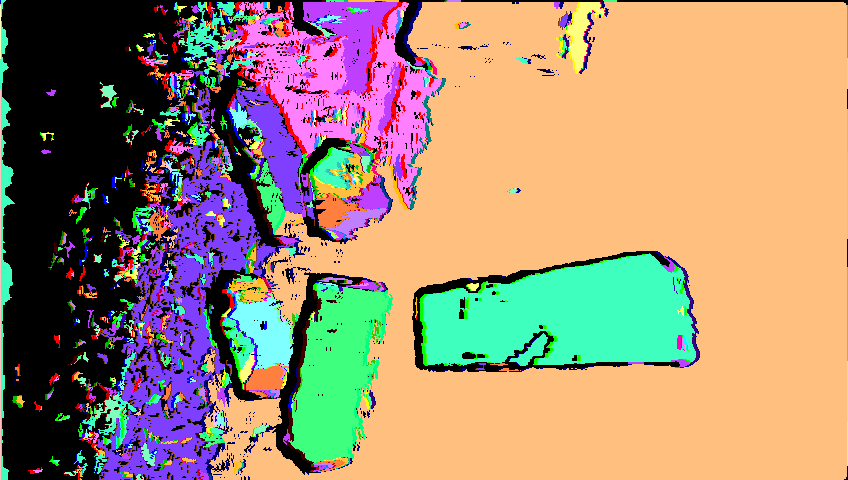
\includegraphics[width = \linewidth]{pictures/obr10_grad.png}
    \caption{Výsledek segmentace obrazu podle velikosti derivace výšky.}
    \label{fig:sobel_segment}
\end{figure}

\subsection{Detekce objektů ze segmentovaného obrazu}
Stejně jako při segmentaci obrazu, tak i zde bylo vyzkoušeno několik algoritmů. Některé z nich byly nastaveny na detekci za zjednodušujících podmínek a nabízí tak nižší výpočetní náročnost při stejné přesnosti detekce. Vstupem všech prezentovaných algoritmů bude segmentovaný obraz jako je například obrázek \ref{fig:height_map}. Tedy vstupem je presketivně deformovaný púdorys jednotlivých cihel.

\subsubsection{Detekce pomocí nejmenší ohraničujícího obdélníku}
\label{sec:bounding_rect}
V tomto algoritmu předpokládáme, že cihly se navzájem nedotýkají, popřípadě se dotýkají pouze po celé délce navzájem si odpovídajících stěn.

Nejprve je na obraz použita morfologická operace otevření, viz sekce \ref{sec:morphology}. Pomocí této operace je obraz vyfiltrován a jsou odstraněny body představující šum. Následně jsou nelezeny obrysy  shluků cihel\footnote{Shlukem cihel se myslí skupina cihel, které jsou spojeny dotekem} pomocí Suzukiho algoritmu \cite{suzuki1985topological}, kde jsme využili již implementovaného programu v knihovně OpenCV.

Pomocí průměrového filtru jsou vyhlazena data reprezentujících obrys shluku cihel, resp. jejich výška. Poté je obrys aproximován konvexním obalem, čímž se zmenší počet bodů, kterými popisujeme daný shluk cihel. Tento shluk je deformován prespektivním zkrslením

Obraz horní stěny kvádr nepodléhá prespektivnímu zkreslení, je-li horní stěna kolmá na optickou osu kamery, tedy normálový vektor reprezentující horní stěnu kvádru musí být rovnoběžný s optickou osou kamery. Normálový vektor horní stěny kvádru ležícího na zemi je stejný s normálovým vektorem \tl{n} země, který byl určen v sekci \ref{sec:normal_est}. Natočení země vůči kameře je vnější vnější parametr kamery. Body obrazu můžeme tedy transformovat do jejich projekce na rovinu země pomocí upraveného vzorce \ref{eq:world_to_img} jako \unsure{Bod \tl{x} bude vyjádřen v homogenních souřadnicích a bude mít tedy tvar x,y,z,1 ...mohu rovnici dole zapsat takto? jedná se o korektní převedení rovnice \ref{eq:world_to_img}, nebo musím explicitně vyjádřit \tl{x}?}
\begin{align}
    \mathbf{x} = \begin{bmatrix} \mathbf{I} \\ 0 \end{bmatrix} \mathbf{K}^{-1} \mathbf{R}^{-1}\mathbf{x}_p, \label{eq:pic_to_world}
\end{align}
kde \tl{R} je matice určená pomocí Rodriguezova vzorce \ref{Rodriguez}. Úhel $\theta$ mezi optickou osou a normálovým vektorem byl určen pomocí vztahu \ref{eq:angle_rogrig} a vektor $\tilde{\mathbf{u}}$, kolem které rotace probíhá, pomocí vztahu \ref{eq:vector_rogrig}. Dostaneme body, které představují konvexní obal, zbavené prespektivního zkrslení.

Následně je nalezen nejmenší obdélník, který opisuje tyto body, viz sekce \ref{sec:nejmenší_obdélník}. Obdélník je plně popsán svými rohy. Na tyto rohy aplikujeme transformaci \ref{eq:world_to_img} a dostaneme body v obrazu, které odpovídají ohraničujícímu obdélníku po aplikování prespektivního zkrslení.

Výše uvedený postup se je proveden pro každou skupinu kostek a následně pro každé patro. Hledáme-li projekci patra $n$, pak jsou z dat odstreněny body,které odpovídají patrům $0,...,n -1$ a postup se opakuje od začátku pro všechny skupiny bloků. Výsledek algoritmu je vidět na obrázku \ref{fig:bb_clasic}


\begin{figure}
    \centering
    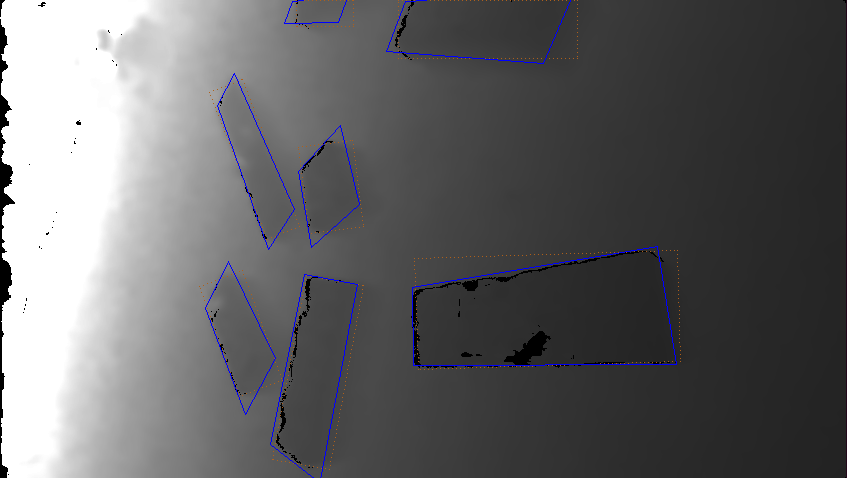
\includegraphics[width = 0.7\linewidth]{pictures/detekce_bb.png}
    \caption{Příklad detekce cihel z hloubkových dat. Modře ohraničující obdélník po odstranění prespektivního zkreslení, hnědě ohraničující obdélník u kterého není bráno v potaz prespektivní zkreslení}
    \label{fig:bb_clasic}
\end{figure}

\subsection{Detekce pomocí RANSAC}
Postup popsaný v sekci \ref{sec:bounding_rect} funguje pouze za zjednodušujících předpokladů a navíc jeho přesnost značně klesá při nesprávném generování stereo párů, jako je vidět na obrázku \ref{fig:point_cloud_grad}. Tato metoda funguje pro všechna natočení cihel a je i velice robustní.

Začneme obdobně jako v sekci \ref{sec:bounding_rect} transformací bodů představující obrysy pomocí vztahu \ref{eq:pic_to_world}. Mezi body, představující prespektivně nezkreslený obrys, najdeme pomocí RANSAC přímku $p_1$. Ta odpovídá některé z delších stěn cihly. Následně je opět použit RANSAC a mezi zbylími body je nelezena přímka $p_2$ rovnoběžná s $p_1$. Tímto dostaneme obě protější stěny cihly. Hledání zbylých 2 kratších stěn je nerealizovatelné i pomocí RANSAC algoritmu, jelikož tyto stěny jsou daleko kratší a tedy reprezentovány méně body. Pokud je obraz zašuměn, pak není možné najít přímku odpovídající této stěně.

Kratší stěny cihly tedy určíme následovně. Vybereme ty body, které leží mezi přímkami $p_1$ a $p_2$.Následně tyto body promítneme přímku $p_1$. Výpočet numericky zjednodušíme otočením bodů a přímek o $\theta$, což je úhel sevřený přímkou $p_1$ a osou $x$. Projekcí na přímku $p_1$ se tedy stane vyčtení $x$-ové souřadnice každého bodu.

Následně je pro každý bod $\mathbf{x} \in p_1$ určen počet bodů promítnutých do okolí o velikosti $\epsilon$. Jsou vybrány dva body s nejvyšší hodnotou, tyto jsou ilustrovány na obrázku \ref{fig:RANSAC_line_short} modrou barvou. Těmito body prochází přímky $p_3$ a $p_4$, které jsou kolmé na $p_1$, popřípadě $p_2$ a představují zbylé 2 stěny obdélníku. Rohy obdélníku $r$ se pak určí jako průsečíky přímek $p$.

Nyní se z bodů představující obrys odečtou ty, které popisují obdélník $r$. Pokud počet zbývajících bodů obrysu je větší, než předem určený limit, pak se proces počínaje hledáním přímky opakuje.

Ve chvíli kdy jsou nelezeny všechny obdélníky, jsou tyto stejně jako v sekci \ref{sec:bounding_rect} jeho rohy transformovány zpět do obrazu a celý postup se opakuje pro další shluky a vrstvy cihel.




%\end{figure}
\begin{figure}
    \centering
    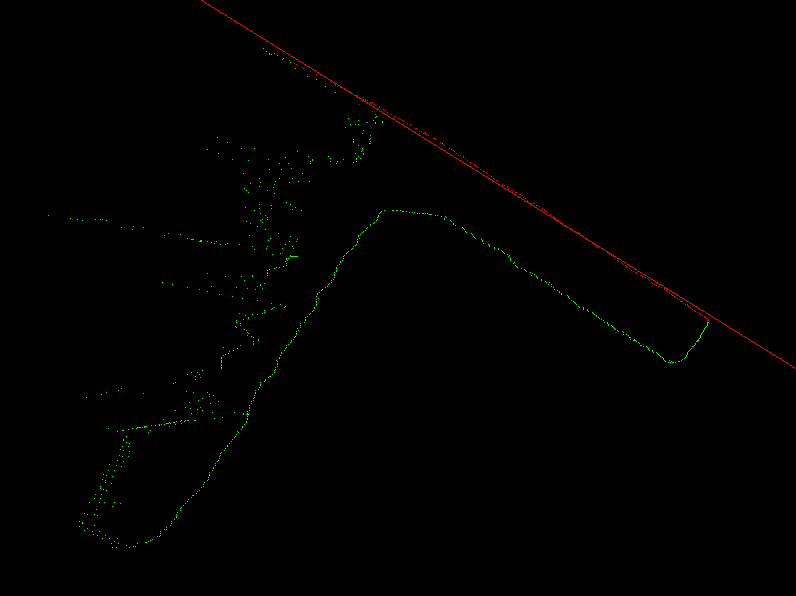
\includegraphics[width = \linewidth]{pictures/ransac_rect_fit1.png}
    \caption{Detekce přímky pomocí RANSAC algoritmu}
    \label{fig:RANSAC_line}
\end{figure}

\begin{figure}
    \centering
    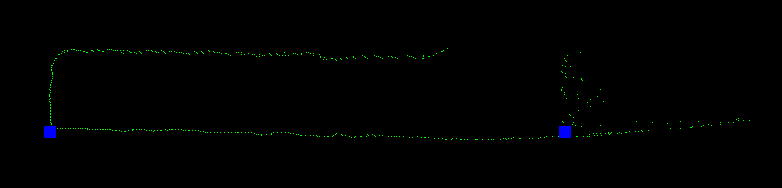
\includegraphics[width = \linewidth]{pictures/crop_ransac_rot.png}
    \caption{Detekce kratších hran cihly.}
    \label{fig:RANSAC_line_short}
\end{figure}

\section{Výsledky}
\label{sec:výsledky}
\todo[inline]{Porovnání jednotlivých výsledků, přesnost + časová náročnost}

\section{Závěr}
\label{sec:závěr}
\todo[inline]{Zhodnocení vhodnosti IntelRealsense pro detekci a zhodnocení prezentovaných algoritmů}


\bibliography{citations}
\bibliographystyle{plain}
\end{document}
